%! TEX program = xelatex

\documentclass{article}
\usepackage[a4paper, margin=3cm]{geometry}
\setlength{\parindent}{0pt}
\setlength{\parskip}{1em}
\usepackage{fontspec}
\setmainfont{Lato}

\usepackage{amsmath,amssymb,amsthm}
%\usepackage{hyperref}
\usepackage{verbatim}
\usepackage{graphicx}
%\usepackage{pgfplots}
%\pgfplotsset{compat=1.16}

\title{}
\author{Mikael Myyrä}
\date{}

\begin{document}

\section*{1.}

Matriisi $L$ on negatiivisen toisen derivaatan differenssiapproksimaatio
\[
  \begin{bmatrix}
    2 & -1 \\
    -1 & 2 & -1 \\
       & \ddots & \ddots & \ddots \\
       & & -1 & 2 & -1 \\
       & & & -1 & 2 \\
  \end{bmatrix}.
\]

Matlab-funktio matriisin rakentamiseen:

\verbatiminput{w7_1_L.m}

\subsection*{(a)}

Matriisin kolme keskimmäistä diagonaalia on ei-nollia ja loput alkiot nollia.
Kun hilaväli pienenee ja matriisin koko kasvaa, niin diagonaalisen nauhan
ulkopuolella olevien alkioiden määrä kasvaa nopeammin kuin siihen kuuluvien
alkioiden määrä, eli täyttöaste pienenee matriisin kasvaessa. Alkioiden määrä
yhteensä on $N^2$ ja kolmella diagonaalilla olevien alkioiden määrä on
$N + 2(N - 1)$.

Esimerkki \verb#spy(L)#:n tuottamasta kuvasta:

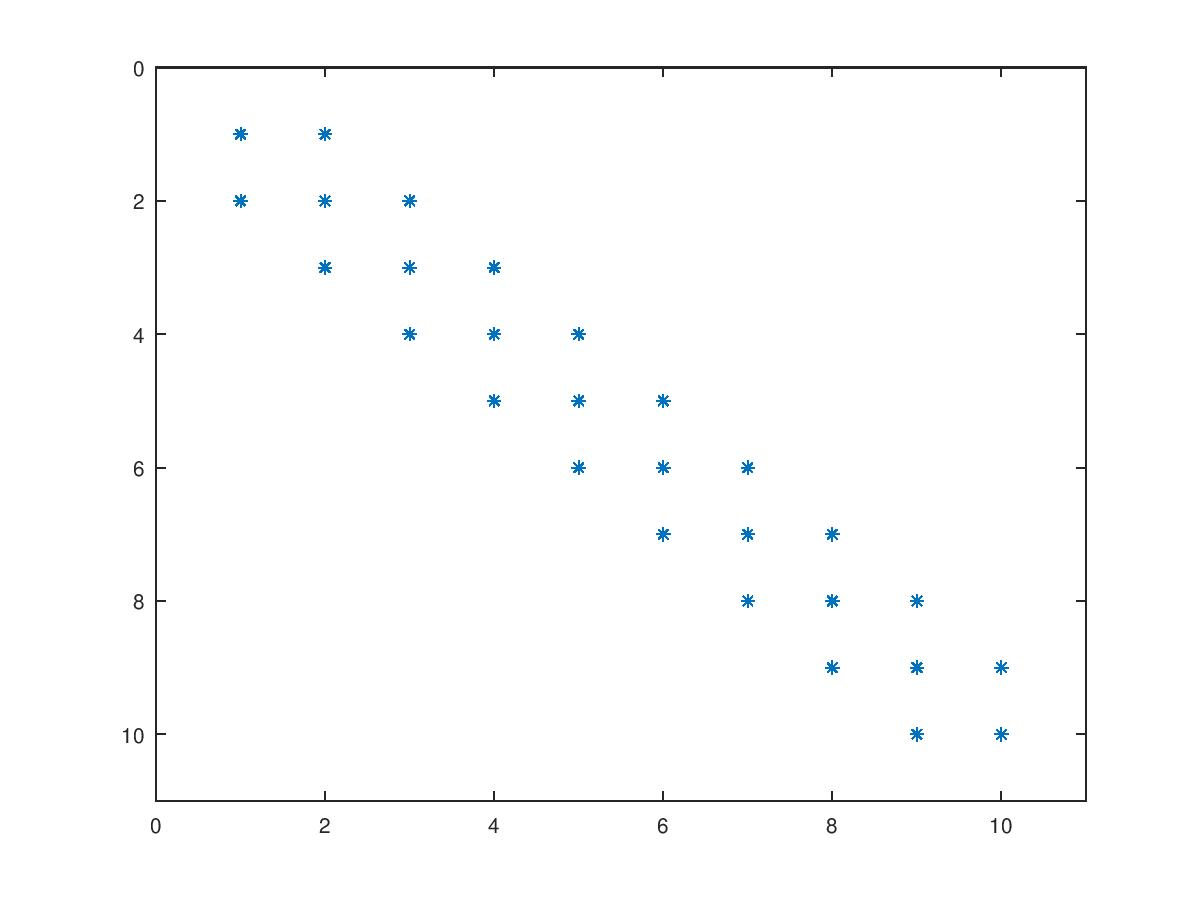
\includegraphics[width=350pt]{w7_1a.jpg}

\subsection*{(b)}

Artikkelin kaava ominaisarvoille on
\[
  \lambda = 4\sin^2 \frac{k\pi}{2(n+1)}, \quad k = 1,2,\dots,n.
\]
Rakensin Octaven interktiivisessa tulkissa kaavan mukaisen vektorin. Sen ja
\verb#eig(L)#:n erotus on likimain nolla, joten ne ovat samat (liukulukujen
tarkkuuden puitteissa).

\subsection*{(c)}

Ominaisvektorien kaava on
\[
  v_i^{(j)} = \sin \Big(\frac{ij\pi}{N+1}\Big), \quad i,j = 1,\dots,N.
\]
Samoin kuin edellisessä kohdassa, rakensin näistä matriisin Octaven
interktiivisessa tulkissa. Sain ensin eri matriisin kuin \verb#eig(L)#:stä,
syynä, että kaavasta saadaan ei-normalisoituja vektoreita. Normalisoinnin
jälkeen matriisit olivat samat.

\newpage
\section*{2.}

\[
  -\Delta u(\mathbf{x}) = 2\pi^2 \sin(\pi x_1) \sin(\pi x_2),
  \quad \mathbf{x} \in \Omega = (0, 1) \times (0, 1)
\]

Kerrotaan funktiolla $v \in H_0^1(\Omega)$ ja integroidaan alueen $\Omega$ yli:
\[
  -\int_{\Omega} (\nabla \cdot \nabla) u v\,dx
  = 2\pi^2 \int_{\Omega} \sin(\pi x_1) \sin(\pi x_2)v\,dx
\]
Greenin lause:
\[
  \int_{\Omega} \nabla v \cdot \nabla u \,dx
  - \int_{\partial \Omega} v\frac{\partial u}{\partial \mathbf{n}} \,dx
  = 2\pi^2 \int_{\Omega} \sin(\pi x_1) \sin(\pi x_2)v\,dx
\]
Reunalla on kaikkialla ehto $u,v = 0$, joten reunan käyräintegraali häviää.
\[
  \int_{\Omega} \nabla v \cdot \nabla u \,dx
  = 2\pi^2 \int_{\Omega} \sin(\pi x_1) \sin(\pi x_2)v\,dx
\]
Tämä on haluttu heikko muoto.

\newpage
\section*{3.}

\[
  u_h(x) = c_1(1-x) + c_2x(1-x) + c_3x^2(1-x)
\]
Reunaehtojen toteutumiseksi täytyy olla
\[
  u_h(0) = c_1 = 1.
\]
Oikean reunan ehto $u_h(1) = 0$ toteutuu kaikilla kertoimien arvoilla.
Saadaan
\[
  u_h(x) = 1 - x + c_2x(1-x) + c_3x^2(1-x).
\]
Residuaali on
\begin{align*}
  r(x) &= Du_h(x) - f(x) \\
       &= \frac{\partial^2 u_h}{\partial x^2} - x^2 \\
       &= 2c_2 + c_3(2 - 6x) - x^2. \\
\end{align*}
Valitaan painofunktiot $w_j = \frac{\partial u_h}{\partial c_j}$,
eli $w_1 = 0$, $w_2 = 1 - 2x$ ja $w_3 = 2x - x^3$.

$w_2$:lla saadaan painotetun residuaalin menetelmästä yhtälö
\begin{align*}
  \int_0^1 w_2r(x)\,dx &= 0 \\
  \int_0^1 (1-2x)(2c_2 + c_3(2 - 6x) - x^2)\,dx &= 0 \\
  \int_0^1 (c_2(2 - 4x) + c_3(2 - 10x + 12x^2) - x^2 + 2x^3) \,dx &= 0 \\
  \int_0^1 (2c_2 + 2c_3 + (-4c_2 - 10c_3)x + (12c_3 - 1)x^2 + 2x^3)\,dx &= 0 \\
  \Big[(2c_2 + 2c_3)x + (-2c_2 - 5c_3)x^2 + (4c_3 - \frac{1}{3})x^2 + \frac{1}{2}x^4\Big]_{x=0}^{x=1} &= 0 \\
  2c_2 + 2c_3 - 2c_2 - 5c_3 + 4c_3 - \frac{1}{3} + \frac{1}{2} &= 0 \\
  c_3 &= -\frac{1}{6} \\
\end{align*}
Tästä saatiin suoraan $c_3$. Sijoitetaan se ja ratkaistaan vastaava yhtälö $w_3$:lla:
\begin{align*}
  \int_0^1 w_3r(x)\,dx &= 0 \\
  \int_0^1 (2x - x^3)(2c_2 + \frac{1}{3} - x - x^2)\,dx &= 0 \\
  \int_0^1 ((4c_2 + \frac{2}{3})x - 2x^2 - 2x^3 - ((2c_2 + \frac{1}{3})x^3 - x^4 - x^5)\,dx &= 0 \\
  \int_0^1 ((4c_2 + \frac{2}{3})x - 2x^2 - (\frac{7}{3} + 2c_2)x^3 + x^4 + x^5)\,dx &= 0 \\
  \Big[(2c_2 + \frac{1}{3})x^2 - \frac{2}{3}x^3 - (\frac{7}{12} + \frac{1}{2})x^4
      + \frac{1}{5}x^5 + \frac{1}{6}x^6\Big]_{x=0}^{x=1} &= 0 \\
  2c_2 + \frac{1}{3} - \frac{2}{3} - \frac{7}{12} - \frac{1}{2} + \frac{1}{5} + \frac{1}{6} &= 0 \\
  c_2 - \frac{1}{6} - \frac{7}{24} - \frac{1}{4} + \frac{1}{10} + \frac{1}{12} &= 0 \\
  c_2 - \frac{15}{24} + \frac{1}{10} &= 0 \\
  c_2 &= \frac{21}{40} \\
\end{align*}

Vastaus: $c_1 = 1$, $c_2 = -\frac{1}{6}$ ja $c_3 = \frac{21}{40}$.

\end{document}
